\documentclass[tikz,border=6pt]{standalone}
\usepackage{pgfplots}
\pgfplotsset{compat=1.18}
\begin{document}
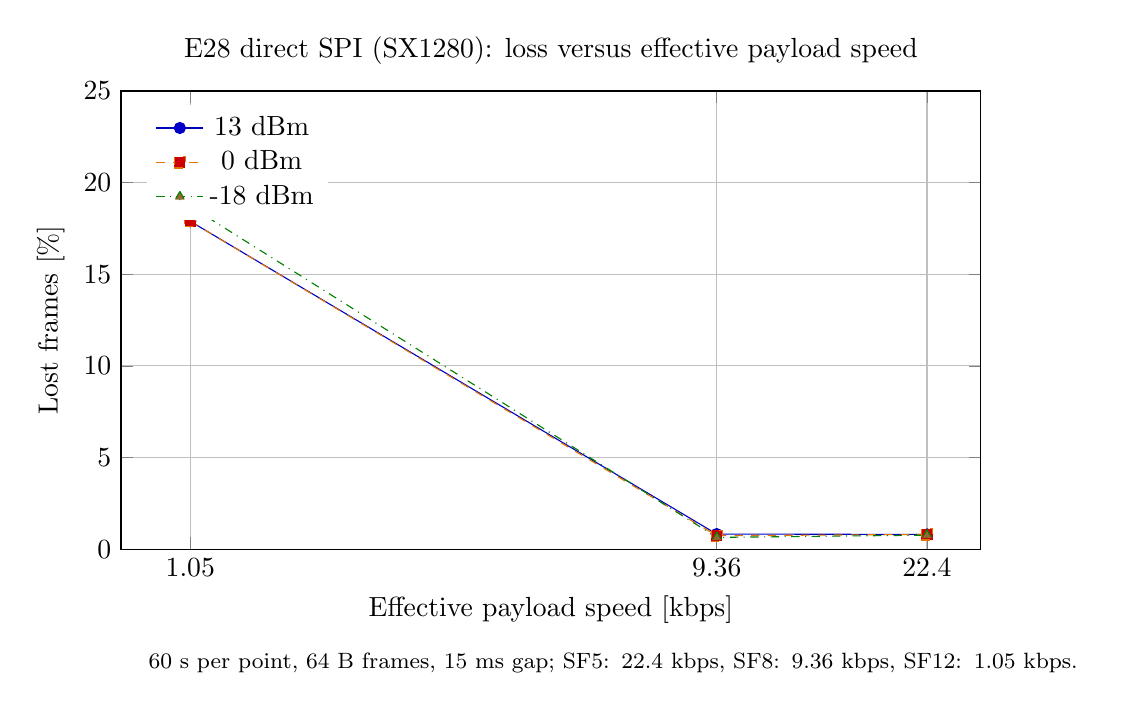
\begin{tikzpicture}
\begin{axis}[width=12.5cm,height=7.4cm,
 title={E28 direct SPI (SX1280): loss versus effective payload speed},xmode=log,xmin=0.7872,xmax=28.0213333,ymin=0,ymax=25,
 xtick={1.0496,9.35537778,22.4113778},xticklabels={1.05,9.36,22.4},
 xlabel={Effective payload speed [kbps]},ylabel={Lost frames [\%]},grid=both,legend style={draw=none,at={(0.03,0.97)},anchor=north west}]
\addplot+[blue!75!black,solid,mark=*] coordinates {(1.0496,17.8861789) (9.35253333,0.821167883) (22.4170667,0.79939094)};
\addlegendentry{13 dBm}
\addplot+[orange!90!black,dashed,mark=square*] coordinates {(1.0496,17.8861789) (9.35253333,0.729927007) (22.4085333,0.799695354)};
\addlegendentry{0 dBm}
\addplot+[green!50!black,dashdotted,mark=triangle*] coordinates {(1.0496,18.699187) (9.36106667,0.63810392) (22.4085333,0.761614623)};
\addlegendentry{-18 dBm}
\end{axis}
\node[font=\footnotesize,align=center,text width=12cm] at (6.25,-1.45) {60 s per point, 64 B frames, 15 ms gap; SF5: 22.4 kbps, SF8: 9.36 kbps, SF12: 1.05 kbps.};
\end{tikzpicture}
\end{document}
